\paragraph{Конвертация информационной модели в FBX-формат}

На первой стадии обработки производится преобразование формата модели.
Как было сказано в разделе~\ref{subsections:DomainModel},
исходный RVT-формат является проприетарной закрытой разработкой
компании Autodesk Inc., хранящей данные в бинарном формате,
что сильно затрудняет разработку парсеров для этого формата.
Помимо этого, Autodesk использует свой формат графических материалов,
которые также плохо-поддерживаются современными графическими фреймворками.

Наиболее эффективными инструментами по работе с форматами
ком\-па\-нии Auto\-desk Inc. являются её же разработки,
поэтому для выполнения преобразования был выбран редактор 3ds~Max.
3ds~Max обладает всей требуемой функциональностью, но, к сожалению,
его программный интерфейс (API) не обладает полным покрытием этой функциональности,
поэтому этот этап не удалось полностью автоматизировать при разработке прототипа.

Использование 3ds~Max для конвертации предполагает следующие шаги:

\begin{enumerate}
    \item {
        Загрузка исходной информационной модели.

        Для загрузки используется инструмент File Link Manager
        (рисунок~\ref{figure:3DCMax-FileLinkManager}),
        позволяющий загружать в 3ds~Max файлы форматов DWG, DXF, FBX и RVT.
        \begin{figure}[!htp]
            \centering
            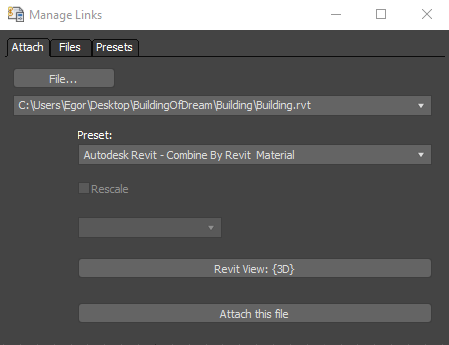
\includegraphics[width=0.5\textwidth, frame]{images/3DSMax-FLM.png}
            \caption{File Link Manager}
            \label{figure:3DCMax-FileLinkManager}
        \end{figure}
        Для загрузки необходимо выбрать загружаемый файл (Attach/File...),
        а затем выбрать одну из предустановленных опций загрузки (Preset).
        Всего на данный момент существует 5 опций,
        но в рамках прототипа нас интересуют только 2:

        \begin{itemize}
            \item {
                Autodesk Revit - Do Not Combine Entities

                При импорте с этой опцией отдельные элементы информационной модели
                будут иметь отдельные полигональные сетки, что в дальнейшем
                позволит полностью сохранить всю атрибутивную информацию.
                Недостатком этой опции является низкая финальная производительность
                и большее использование памяти для хранения такой модели
                на диске и в оперативной памяти.
            }
            \item {
                Autodesk Revit - Combine By Revit Category

                При импорте с данной опцией элементы модели, относящиеся к одной категории,
                будут объединены в одну полигональную сетку, что можно считать
                статическим батчингом модели (описано ранее
                в разделе~\ref{subsections:Optimization}).
                Такой вариант был выбран предпочтительным,
                хотя при нём неизбежно утрачивается
                значительная часть атрибутивной информации.
            }
        \end{itemize}

        После этого необходимо завершить загрузку:
        Attach/Attach this file + Files/Bind...
    }
    \item {
        Конвертация графических материалов.
        
        Для конвертации графических материалов сцены
        был использован инструмент Scene Converter (рисунок~\ref{figure:3DCMax-SceneConverter}).
        \begin{figure}[!htp]
            \centering
            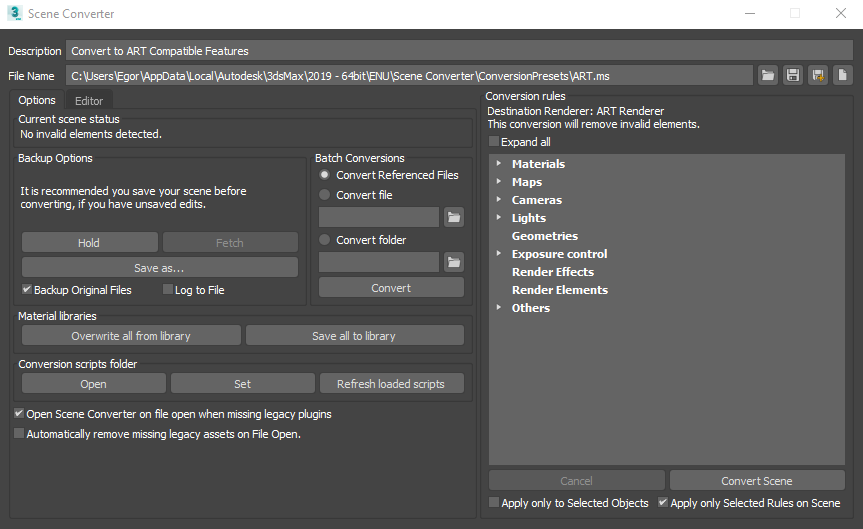
\includegraphics[width=0.8\textwidth, frame]{images/3DSMax-SC.png}
            \caption{Scene Converter}
            \label{figure:3DCMax-SceneConverter}
        \end{figure}
        Scene Converter позволяет конвертировать различные элементы сцены,
        применяя определенные правила.
        В данном случае нас интересует правило
        ``Autodesk Material to Physical Material'',
        преобразующее проприетарные графические материалы Autodesk,
        в широко используемые графические материалы,
        основанные на физических свойствах поверхности.
    }
    \item {
        Сохранение FBX модели.

        В завершение необходимо экспортировать полученную модель в FBX формате
        (рисунок~\ref{figure:3DCMax-Export}).
        \begin{figure}[!htp]
            \centering
            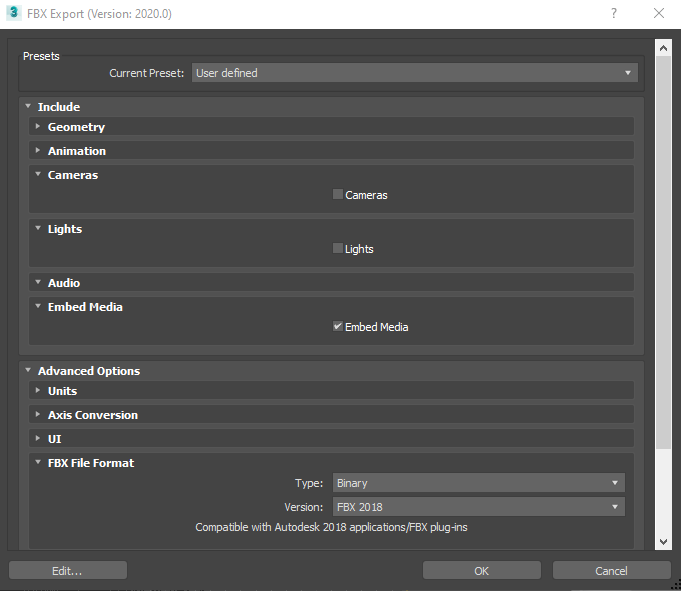
\includegraphics[width=0.7\textwidth, frame]{images/3DSMax-Export.png}
            \caption{FBX Export}
            \label{figure:3DCMax-Export}
        \end{figure}
        При сохранении необходимо исключить все анимации, камеры
        и источники света, если они присутствуют в оригинальной информационной модели,
        но сохранить встроенные медиа-данные.
    }
\end{enumerate}
